% Options for packages loaded elsewhere
\PassOptionsToPackage{unicode}{hyperref}
\PassOptionsToPackage{hyphens}{url}
%
\documentclass[
  8pt,
  ignorenonframetext,
]{beamer}
\usepackage{pgfpages}
\setbeamertemplate{caption}[numbered]
\setbeamertemplate{caption label separator}{: }
\setbeamercolor{caption name}{fg=normal text.fg}
\beamertemplatenavigationsymbolsempty
% Prevent slide breaks in the middle of a paragraph
\widowpenalties 1 10000
\raggedbottom
\setbeamertemplate{part page}{
  \centering
  \begin{beamercolorbox}[sep=16pt,center]{part title}
    \usebeamerfont{part title}\insertpart\par
  \end{beamercolorbox}
}
\setbeamertemplate{section page}{
  \centering
  \begin{beamercolorbox}[sep=12pt,center]{part title}
    \usebeamerfont{section title}\insertsection\par
  \end{beamercolorbox}
}
\setbeamertemplate{subsection page}{
  \centering
  \begin{beamercolorbox}[sep=8pt,center]{part title}
    \usebeamerfont{subsection title}\insertsubsection\par
  \end{beamercolorbox}
}
\AtBeginPart{
  \frame{\partpage}
}
\AtBeginSection{
  \ifbibliography
  \else
    \frame{\sectionpage}
  \fi
}
\AtBeginSubsection{
  \frame{\subsectionpage}
}
\usepackage{amsmath,amssymb}
\usepackage{iftex}
\ifPDFTeX
  \usepackage[T1]{fontenc}
  \usepackage[utf8]{inputenc}
  \usepackage{textcomp} % provide euro and other symbols
\else % if luatex or xetex
  \usepackage{unicode-math} % this also loads fontspec
  \defaultfontfeatures{Scale=MatchLowercase}
  \defaultfontfeatures[\rmfamily]{Ligatures=TeX,Scale=1}
\fi
\usepackage{lmodern}
\usetheme[]{CambridgeUS}
\ifPDFTeX\else
  % xetex/luatex font selection
\fi
% Use upquote if available, for straight quotes in verbatim environments
\IfFileExists{upquote.sty}{\usepackage{upquote}}{}
\IfFileExists{microtype.sty}{% use microtype if available
  \usepackage[]{microtype}
  \UseMicrotypeSet[protrusion]{basicmath} % disable protrusion for tt fonts
}{}
\makeatletter
\@ifundefined{KOMAClassName}{% if non-KOMA class
  \IfFileExists{parskip.sty}{%
    \usepackage{parskip}
  }{% else
    \setlength{\parindent}{0pt}
    \setlength{\parskip}{6pt plus 2pt minus 1pt}}
}{% if KOMA class
  \KOMAoptions{parskip=half}}
\makeatother
\usepackage{xcolor}
\newif\ifbibliography
\usepackage{color}
\usepackage{fancyvrb}
\newcommand{\VerbBar}{|}
\newcommand{\VERB}{\Verb[commandchars=\\\{\}]}
\DefineVerbatimEnvironment{Highlighting}{Verbatim}{commandchars=\\\{\}}
% Add ',fontsize=\small' for more characters per line
\usepackage{framed}
\definecolor{shadecolor}{RGB}{248,248,248}
\newenvironment{Shaded}{\begin{snugshade}}{\end{snugshade}}
\newcommand{\AlertTok}[1]{\textcolor[rgb]{0.94,0.16,0.16}{#1}}
\newcommand{\AnnotationTok}[1]{\textcolor[rgb]{0.56,0.35,0.01}{\textbf{\textit{#1}}}}
\newcommand{\AttributeTok}[1]{\textcolor[rgb]{0.13,0.29,0.53}{#1}}
\newcommand{\BaseNTok}[1]{\textcolor[rgb]{0.00,0.00,0.81}{#1}}
\newcommand{\BuiltInTok}[1]{#1}
\newcommand{\CharTok}[1]{\textcolor[rgb]{0.31,0.60,0.02}{#1}}
\newcommand{\CommentTok}[1]{\textcolor[rgb]{0.56,0.35,0.01}{\textit{#1}}}
\newcommand{\CommentVarTok}[1]{\textcolor[rgb]{0.56,0.35,0.01}{\textbf{\textit{#1}}}}
\newcommand{\ConstantTok}[1]{\textcolor[rgb]{0.56,0.35,0.01}{#1}}
\newcommand{\ControlFlowTok}[1]{\textcolor[rgb]{0.13,0.29,0.53}{\textbf{#1}}}
\newcommand{\DataTypeTok}[1]{\textcolor[rgb]{0.13,0.29,0.53}{#1}}
\newcommand{\DecValTok}[1]{\textcolor[rgb]{0.00,0.00,0.81}{#1}}
\newcommand{\DocumentationTok}[1]{\textcolor[rgb]{0.56,0.35,0.01}{\textbf{\textit{#1}}}}
\newcommand{\ErrorTok}[1]{\textcolor[rgb]{0.64,0.00,0.00}{\textbf{#1}}}
\newcommand{\ExtensionTok}[1]{#1}
\newcommand{\FloatTok}[1]{\textcolor[rgb]{0.00,0.00,0.81}{#1}}
\newcommand{\FunctionTok}[1]{\textcolor[rgb]{0.13,0.29,0.53}{\textbf{#1}}}
\newcommand{\ImportTok}[1]{#1}
\newcommand{\InformationTok}[1]{\textcolor[rgb]{0.56,0.35,0.01}{\textbf{\textit{#1}}}}
\newcommand{\KeywordTok}[1]{\textcolor[rgb]{0.13,0.29,0.53}{\textbf{#1}}}
\newcommand{\NormalTok}[1]{#1}
\newcommand{\OperatorTok}[1]{\textcolor[rgb]{0.81,0.36,0.00}{\textbf{#1}}}
\newcommand{\OtherTok}[1]{\textcolor[rgb]{0.56,0.35,0.01}{#1}}
\newcommand{\PreprocessorTok}[1]{\textcolor[rgb]{0.56,0.35,0.01}{\textit{#1}}}
\newcommand{\RegionMarkerTok}[1]{#1}
\newcommand{\SpecialCharTok}[1]{\textcolor[rgb]{0.81,0.36,0.00}{\textbf{#1}}}
\newcommand{\SpecialStringTok}[1]{\textcolor[rgb]{0.31,0.60,0.02}{#1}}
\newcommand{\StringTok}[1]{\textcolor[rgb]{0.31,0.60,0.02}{#1}}
\newcommand{\VariableTok}[1]{\textcolor[rgb]{0.00,0.00,0.00}{#1}}
\newcommand{\VerbatimStringTok}[1]{\textcolor[rgb]{0.31,0.60,0.02}{#1}}
\newcommand{\WarningTok}[1]{\textcolor[rgb]{0.56,0.35,0.01}{\textbf{\textit{#1}}}}
\usepackage{graphicx}
\makeatletter
\def\maxwidth{\ifdim\Gin@nat@width>\linewidth\linewidth\else\Gin@nat@width\fi}
\def\maxheight{\ifdim\Gin@nat@height>\textheight\textheight\else\Gin@nat@height\fi}
\makeatother
% Scale images if necessary, so that they will not overflow the page
% margins by default, and it is still possible to overwrite the defaults
% using explicit options in \includegraphics[width, height, ...]{}
\setkeys{Gin}{width=\maxwidth,height=\maxheight,keepaspectratio}
% Set default figure placement to htbp
\makeatletter
\def\fps@figure{htbp}
\makeatother
\setlength{\emergencystretch}{3em} % prevent overfull lines
\providecommand{\tightlist}{%
  \setlength{\itemsep}{0pt}\setlength{\parskip}{0pt}}
\setcounter{secnumdepth}{-\maxdimen} % remove section numbering
\ifLuaTeX
  \usepackage{selnolig}  % disable illegal ligatures
\fi
\IfFileExists{bookmark.sty}{\usepackage{bookmark}}{\usepackage{hyperref}}
\IfFileExists{xurl.sty}{\usepackage{xurl}}{} % add URL line breaks if available
\urlstyle{same}
\hypersetup{
  pdftitle={Intro to programming 3},
  hidelinks,
  pdfcreator={LaTeX via pandoc}}

\title{Intro to programming 3}
\author{Henri Vandendriessche\\
\href{mailto:henri.vandendriessche@ens.fr}{\nolinkurl{henri.vandendriessche@ens.fr}}}
\date{2023-10-03}

\begin{document}
\frame{\titlepage}

\begin{frame}[fragile]{Terminal cheat sheet reminder}
\protect\hypertarget{terminal-cheat-sheet-reminder}{}
\begin{itemize}
\item
  Bash commands to navigate directories

  \begin{itemize}
  \tightlist
  \item
    Print Working Directory. Print the path of the current directory
  \end{itemize}

\begin{Shaded}
\begin{Highlighting}[]
\BuiltInTok{pwd}
\end{Highlighting}
\end{Shaded}

  \begin{itemize}
  \tightlist
  \item
    List all files of the current directory
  \end{itemize}

\begin{Shaded}
\begin{Highlighting}[]
\FunctionTok{ls}\NormalTok{ folder}
\end{Highlighting}
\end{Shaded}

  \begin{itemize}
  \tightlist
  \item
    Moving into folder1 and subfolder2 at once.
  \end{itemize}

\begin{Shaded}
\begin{Highlighting}[]
\BuiltInTok{cd}\NormalTok{ folder1/subfolder2}
\end{Highlighting}
\end{Shaded}

  \begin{itemize}
  \tightlist
  \item
    Moving out of a directory
  \end{itemize}

\begin{Shaded}
\begin{Highlighting}[]
\BuiltInTok{cd}\NormalTok{ ..}
\end{Highlighting}
\end{Shaded}

  \begin{itemize}
  \tightlist
  \item
    Going back and forth in the directory tree
  \end{itemize}

\begin{Shaded}
\begin{Highlighting}[]
\BuiltInTok{cd}\NormalTok{ ../../folder1/subfolder1}
\end{Highlighting}
\end{Shaded}

  \begin{itemize}
  \tightlist
  \item
    Going back to the root directory
  \end{itemize}

\begin{Shaded}
\begin{Highlighting}[]
\BuiltInTok{cd}\NormalTok{ \textasciitilde{}}
\end{Highlighting}
\end{Shaded}
\item
  ``\textbf{Tab}'' to use the auto-completion
\item
  \textbf{Ctrl + C} to stop a program execution
\item
  ``\textbf{Upper arrow}'' to see last commands
\item
  Many more bash commands to use\ldots{}
\end{itemize}
\end{frame}

\begin{frame}{So far}
\protect\hypertarget{so-far}{}
\begin{itemize}
\item
  Python
\item
  Data types:

  \begin{itemize}
  \tightlist
  \item
    integer
  \item
    float
  \item
    string
  \item
    boolean
  \end{itemize}
\item
  \textbf{If}, \textbf{For} and \textbf{While} loops:

  \begin{itemize}
  \tightlist
  \item
    syntax
  \item
    indentation
  \end{itemize}
\item
  Data collections:

  \begin{itemize}
  \tightlist
  \item
    list
  \item
    tuple
  \item
    set
  \item
    dictionary
  \end{itemize}
\end{itemize}
\end{frame}

\begin{frame}{Today}
\protect\hypertarget{today}{}
\begin{itemize}
\item
  Python standard library
\item
  Random numbers and number choices
\item
  Exercises
\end{itemize}
\end{frame}

\begin{frame}{Python standard library 1/3}
\protect\hypertarget{python-standard-library-13}{}
\begin{itemize}[<+->]
\tightlist
\item
  Python's standard library is incredibly extensive, offering a wide
  range of facilities, as indicated by the comprehensive table of
  contents listed below:

  \begin{itemize}[<+->]
  \tightlist
  \item
    \url{https://docs.python.org/3/library/index.html}
  \end{itemize}
\end{itemize}

\begin{itemize}[<+->]
\tightlist
\item
  The ``Python library'' encompasses various types of components.
\end{itemize}

\begin{itemize}[<+->]
\tightlist
\item
  It includes data types that are typically considered part of the core
  of a language, such as numbers and lists.
\end{itemize}

\begin{itemize}[<+->]
\tightlist
\item
  The library also contains built-in functions and exceptions---objects
  that can be used by all Python code without the need for an import
  statement. While some of these are defined by the core language, many
  are not essential for the core semantics and are only described in
  this documentation.
\end{itemize}

\begin{itemize}[<+->]
\tightlist
\item
  This manual, available at
  (\url{https://docs.python.org/3/library/index.html}) is organized
  ``from the inside out.'' It first describes the built-in functions,
  data types, and exceptions and finally covers the modules, grouped in
  chapters of related modules.
\end{itemize}
\end{frame}

\begin{frame}{Python standard library 2/3}
\protect\hypertarget{python-standard-library-23}{}
\begin{itemize}[<+->]
\tightlist
\item
  One of Python's greatest strengths is its extensive standard library.
\end{itemize}

\begin{itemize}[<+->]
\tightlist
\item
  Python supports many internet protocols.
\end{itemize}

\begin{itemize}[<+->]
\tightlist
\item
  Python includes modules for working with relational databases.
\end{itemize}

\begin{itemize}[<+->]
\tightlist
\item
  Python also offers modules for creating graphical user interfaces.
\end{itemize}

\begin{itemize}[<+->]
\tightlist
\item
  Python comes with a wide range of built-in functions. You can find a
  list of these functions here
  (\url{https://docs.python.org/3/library/functions.html})
\end{itemize}

\begin{itemize}[<+->]
\tightlist
\item
  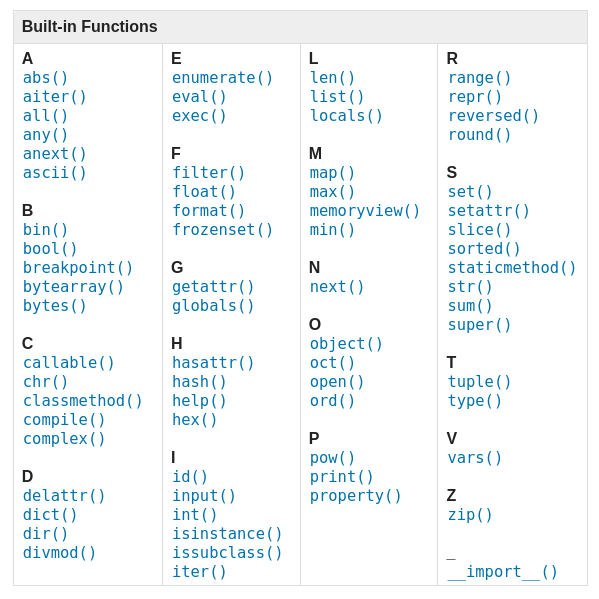
\includegraphics{/home/dbhenri/Documents/Cours python/PCBS/slides/intro-to-programming/2022/3rd class/built_in_functions.png}
\end{itemize}
\end{frame}

\begin{frame}{Python standard library 3/3}
\protect\hypertarget{python-standard-library-33}{}
\begin{itemize}
\item
  In addition to the standard library, Python Package Index (PyPI), the
  official repository for third-party Python software, contains over 485
  000 packages (as of September 2023)
\item
  Example of famous third-party Python packages on PyPi:

  \begin{itemize}
  \tightlist
  \item
    Pandas (data analysis/datascience)
  \item
    Matplotlib (data exploration and vizualization)
  \item
    Seaborn (high end graphics and drawing)
  \item
    Scikit-learn (data analysis, machine learning)
  \end{itemize}
\end{itemize}
\end{frame}

\begin{frame}{Python module - example of \textbf{Random} 1/4}
\protect\hypertarget{python-module---example-of-random-14}{}
-Python includes a multitude of modules in its standard library,
covering a wide range of subjects and problem domains, including network
operations, text processing, mathematics, file and directory access,
cryptography, and more.

\url{https://docs.python.org/3/library/index.html}

\begin{itemize}
\tightlist
\item
  The standard library includes a dedicated module for random
  (pseudo-random) number generation.
\end{itemize}

\url{https://docs.python.org/3/library/random.html}
\end{frame}

\begin{frame}[fragile]{Python module - example of \textbf{Random} 2/4}
\protect\hypertarget{python-module---example-of-random-24}{}
\begin{itemize}
\tightlist
\item
  There are several ways to import a python module
\end{itemize}

\begin{Shaded}
\begin{Highlighting}[]
\ImportTok{import}\NormalTok{ random }\CommentTok{\# import random}
\NormalTok{int\_list }\OperatorTok{=}\NormalTok{[}\DecValTok{1}\NormalTok{,}\DecValTok{2}\NormalTok{,}\DecValTok{3}\NormalTok{]}
\NormalTok{random.shuffle(int\_list)}\CommentTok{\# from that object you have to access all the functions}
\BuiltInTok{print}\NormalTok{(int\_list)}
\end{Highlighting}
\end{Shaded}

\begin{verbatim}
## [1, 3, 2]
\end{verbatim}

\begin{Shaded}
\begin{Highlighting}[]
\ImportTok{import}\NormalTok{ random }\ImportTok{as}\NormalTok{ rand }\CommentTok{\# import random using a custom local name }
\NormalTok{rand.shuffle(int\_list) }\CommentTok{\# from that object you have to access all the functions}
\BuiltInTok{print}\NormalTok{(int\_list)}
\end{Highlighting}
\end{Shaded}

\begin{verbatim}
## [3, 2, 1]
\end{verbatim}

\begin{Shaded}
\begin{Highlighting}[]
\ImportTok{from}\NormalTok{ random }\ImportTok{import}\NormalTok{ shuffle,randint,choice }\CommentTok{\# import only needed function}
\NormalTok{shuffle(int\_list) }\CommentTok{\# use the function directly without object before}
\BuiltInTok{print}\NormalTok{(int\_list)}
\end{Highlighting}
\end{Shaded}

\begin{verbatim}
## [3, 1, 2]
\end{verbatim}

\begin{Shaded}
\begin{Highlighting}[]
\ImportTok{from}\NormalTok{ random }\ImportTok{import} \OperatorTok{*} \CommentTok{\# import all the functions bundled inside Random at once}
\NormalTok{shuffle(int\_list)}
\BuiltInTok{print}\NormalTok{(int\_list)}
\end{Highlighting}
\end{Shaded}

\begin{verbatim}
## [2, 1, 3]
\end{verbatim}
\end{frame}

\begin{frame}[fragile]{Python module - example of \textbf{Random} 3/4}
\protect\hypertarget{python-module---example-of-random-34}{}
\begin{Shaded}
\begin{Highlighting}[]
\ImportTok{from}\NormalTok{ random }\ImportTok{import} \OperatorTok{*}

\BuiltInTok{print}\NormalTok{(randint(}\DecValTok{1}\NormalTok{, }\DecValTok{100}\NormalTok{))    }\CommentTok{\# Pick a random integer between 1 and 100.}
\end{Highlighting}
\end{Shaded}

\begin{verbatim}
## 95
\end{verbatim}

\begin{Shaded}
\begin{Highlighting}[]
\BuiltInTok{print}\NormalTok{(uniform(}\DecValTok{1}\NormalTok{, }\DecValTok{100}\NormalTok{))    }\CommentTok{\# Pick a random float between 1 and 100.}
\end{Highlighting}
\end{Shaded}

\begin{verbatim}
## 39.62301668245445
\end{verbatim}

\begin{Shaded}
\begin{Highlighting}[]
\CommentTok{\# prints a random value from the list}
\NormalTok{list1 }\OperatorTok{=}\NormalTok{ [}\DecValTok{1}\NormalTok{, }\DecValTok{2}\NormalTok{, }\DecValTok{3}\NormalTok{, }\DecValTok{4}\NormalTok{, }\DecValTok{5}\NormalTok{, }\DecValTok{6}\NormalTok{]}
\BuiltInTok{print}\NormalTok{(choice(list1))}
\end{Highlighting}
\end{Shaded}

\begin{verbatim}
## 6
\end{verbatim}

\begin{Shaded}
\begin{Highlighting}[]
\NormalTok{items }\OperatorTok{=}\NormalTok{ [}\DecValTok{1}\NormalTok{, }\DecValTok{2}\NormalTok{, }\DecValTok{3}\NormalTok{, }\DecValTok{4}\NormalTok{, }\DecValTok{5}\NormalTok{, }\DecValTok{6}\NormalTok{, }\DecValTok{7}\NormalTok{, }\DecValTok{8}\NormalTok{, }\DecValTok{9}\NormalTok{, }\DecValTok{10}\NormalTok{]}
\NormalTok{y }\OperatorTok{=}\NormalTok{ sample(items, }\DecValTok{4}\NormalTok{)    }\CommentTok{\# Pick 4 random items from the list}
\BuiltInTok{print}\NormalTok{(y)}
\end{Highlighting}
\end{Shaded}

\begin{verbatim}
## [4, 10, 5, 7]
\end{verbatim}
\end{frame}

\begin{frame}[fragile]{Python module - example of \textbf{Random} 4/4}
\protect\hypertarget{python-module---example-of-random-44}{}
\begin{Shaded}
\begin{Highlighting}[]
\CommentTok{\# using randrange() to generate in range from 20}
\CommentTok{\# to 50. The last parameter 3 is step size to skip}
\CommentTok{\# three numbers when selecting.}
\BuiltInTok{print}\NormalTok{(}\StringTok{"A random number from range is : "}\NormalTok{, end}\OperatorTok{=}\StringTok{""}\NormalTok{)}
\end{Highlighting}
\end{Shaded}

\begin{verbatim}
## A random number from range is :
\end{verbatim}

\begin{Shaded}
\begin{Highlighting}[]
\BuiltInTok{print}\NormalTok{(randrange(}\DecValTok{20}\NormalTok{, }\DecValTok{50}\NormalTok{, }\DecValTok{3}\NormalTok{))}
\end{Highlighting}
\end{Shaded}

\begin{verbatim}
## 26
\end{verbatim}
\end{frame}

\begin{frame}{Exercises}
\protect\hypertarget{exercises}{}
\begin{itemize}
\item
  Exercise 1: Lottery pick. Generate 100 random lottery tickets (one
  ticket is a sequence of 5 digits) and pick one winner out of it.
\item
  Exercise 2: write a program that generates a random 10 character long
  password including 6 letters with 2 of them uppercase, 1 digit and 1
  special symbol.
\item
  Exercise 3: Monte Carlo estimation of Pi: one way to estimate the
  value of the pi is to generate a large number of random points in the
  unit square and see how many fall within the unit circle; their
  proportion is an estimate of the area of the circle. See
  \url{https://academo.org/demos/estimating-pi-monte-carlo}. Implement
  the proposed algorithm to estimate the value of pi.
\item
  Exercise 4: Write a program that prints the first N rows of Pascal's
  triangle (see \url{https://www.youtube.com/watch?v=XMriWTvPXHI}).
\end{itemize}
\end{frame}

\end{document}
